\documentclass{article}

\usepackage[utf8]{inputenc}
\usepackage[greek, british]{babel}
\usepackage{alphabeta}
\usepackage{libertine}
\usepackage{csquotes}
\usepackage[backend=biber, sorting=none]{biblatex}
\usepackage{hyperref}
\usepackage{graphicx}
\usepackage{float}
\graphicspath{ {./images/} }

\pagenumbering{arabic}

\addbibresource{refs.bib}

\newcommand{\code}{\texttt}

\title{Εργασία Μηχανικής Μάθησης 2022}
\author{Tsirmpas Dimitris}

\begin{document}
	
\maketitle
	
\section{Λογιστική Παλινδρόμηση}

\subsection{Ερώτημα Δ}
Ο ταξινομητής μας έχει υλοποιηθεί στο αρχείο \code{LogisticRegClassifier.py}. Η πλήρης τεκμηρίωση του μοντέλου, των μεθόδων του και των υπερπαραμέτρων βρίσκεται εκεί με τη μορφή docstrings. Η κανονικοποίηση $L_{2}$ έχει ήδη υλοποιηθεί σε αυτό το αρχείο, αλλά για τους σκοπούς αυτής της ερώτησης θα θέσουμε την υπερπαράμετρο \code{$\lambda$} ως 0, παρακάμπτοντας την.\par

Ο κώδικας για την εκτέλεση του μοντέλου βρίσκεται στο αρχείο \code{run\_logistic.py}. Θα τρέξουμε το μοντέλο με υπερπαραμέτρους \code{iter = 500} και \code{alpha = 0.2}. Το αποτέλεσμα είναι η ακρίβεια εκπαίδευσης να είναι ίση με $0.982$ και η ακρίβεια ελέγχου ίση με $0.981$. Τα πλήρη αποτελέσματα της εκπαίδευσης και του ελέγχου παρουσιάζονται στην εικόνα \ref{logistic_train_test}.

\begin{figure}
	\label{logistic_train_test}
	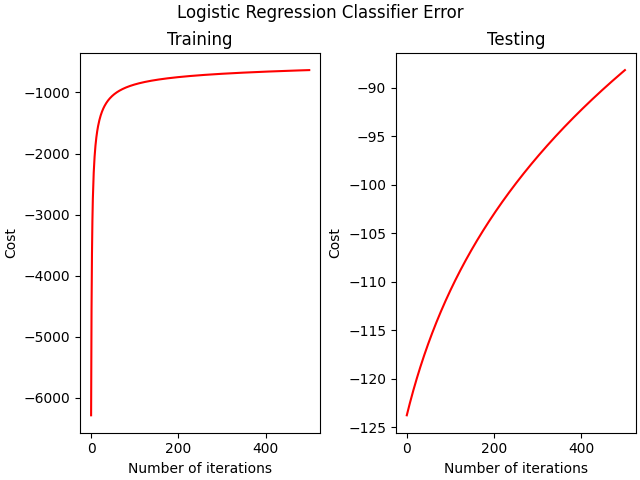
\includegraphics[width=10cm]{logistic_error.png}
	\centering
	\caption{Τα αποτελέσματα της εκπαίδευσης και του ελέγχου στον ταξινομητή μας. Αριστερά: Το κόστος εκπαίδευσης ως συνάρτηση των επαναλήψεων του αλγορίθμου gradient ascent. Δεξία: Το αντίστοιχο κόστος ελέγχου. Υπενθυμίζουμε ότι οι κλίμακες των γραφημάτων δεν είναι ίσες, καθώς ο ήδη εκπαιδευμένος ταξινομητής αρχίζει με πολύ μικρότερο κόστος. }
\end{figure}


\subsection{Ερώτημα Ε}
Επιλέγουμε το διάστημα των \code{$\lambda$} τιμών μας λογαριθμικά, εφόσον η βέλτιστη τιμή κανονικοποίησης είναι πολύ πιο πιθανό να βρίσκεται αρκετά κοντά στο 0. Η λογαριθμική κλίμακα μας επιτρέπει να ψάξουμε πιο πολλές τιμές του \code{$\lambda$} όσο πιο κοντά φτάνουμε στο κάτω όριο αναζήτησης μας, το $10^{4}$.Η προσέγγιση αυτή χρησιμοποιείται και στην πράξη για κανονικοποίηση $L^{2}$ \cite{jerome}\par

Κατά την εκτέλεση του προγράμματος υπάρχει πιθανότητα να εμφανιστούν ειδοποιήσεις για αριθμητική υπερχείλιση. Για αυτό ευθύνεται η επιλογή πολύ μεγάλης τιμής του \code{$\lambda$}, κυρίως στο δίαστημα [8, 10]. Σε αυτό το σημείο η κανονικοποίηση είναι τόσο ισχυρή που αποτρέπει το μοντέλο μας από το να μάθει, και έτσι αυτό μαντεύει πάντα την ίδια κατηγορία.\par

Στην δική μας περίπτωση το μοντέλο, κρατώντας τις υπόλοιπες υπερπαραμέτρους ίσες με το προηγούμενο υποερώτημα, προτιμά την ελάχιστη τιμή κανονικοποίησης \code{$\lambda = 10^{4}$} με ακρίβεια επαλήθευσης ίση με 0.979 και ακρίβεια ελέγχου ίση με 0.981. Παρατηρούμε ότι η ακρίβεια ελέγχου με την επιλεγμένη τιμή \code{$\lambda$} είναι μικρότερη από την αντίστοιχη στο υποερώτημα Δ. Αυτό μας υποδεικνύει είτε ότι η βέλτιστη τιμή βρίσκεται έξω (και πιο συγκεκριμένα πριν) από το διάστημα αναζήτησης μας, είτε ότι για την διαφορά ευθύνεται το στατιστικό σφάλμα. \par

Τα πλήρη αποτελέσματα αναζήτησης της υπερπαραμέτρου παρουσιάζονται στην εικόνα \ref{logistic_lambda_accuracy}.

\begin{figure}
	\label{logistic_lambda_accuracy}
	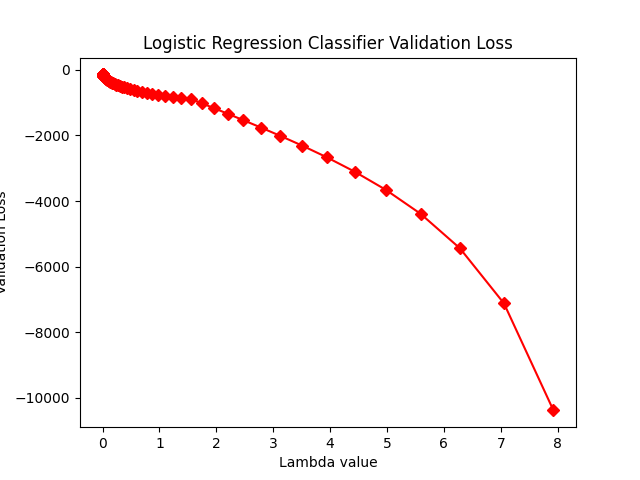
\includegraphics[width=10cm]{logistic_lambda_accuracy.png}
	\centering
	\caption{ Τα αποτελέσματα της αναζήτησης για το βέλτιστο \code{$\lambda$}. Οι ρόμβοι αντιπροσωπεύουν τις τιμές που εξετάσαμε. Παρατηρείστε το πλήθος των τιμών που εξετάστηκαν στην αρχή συγκριτικά με το τέλος του πεδίου αναζήτησής μας.}
\end{figure}

\printbibliography

\end{document}